\documentclass[12pt,titlepage,french]{article}
\usepackage{babel}
\usepackage{graphicx}
\usepackage[margin=2.5cm]{geometry}

\usepackage[hidelinks]{hyperref}
\usepackage{tabularx}
\usepackage[utf8]{inputenc}
\usepackage[T1]{fontenc}
\pagestyle{plain}

\usepackage{booktabs,makecell,tabu}
\usepackage{comment}
\renewcommand\theadfont{\bfseries}

\linespread{1.5}

\newcounter{firstbib}

\begin{document}
%\renewcommand{\thesection}{\arabic{section}} % utilisé pour spécifier la numérotation des sections

\begin{titlepage}
\newcommand{\HRule}{\rule{\linewidth}{0.5mm}}
\center

  
\includegraphics[width=0.45\textwidth]{../../ressources/img_logos/logo_polytech.png}\\[1cm]

  
\includegraphics[width=0.45\textwidth]{../../ressources/img_logos/logo_taglabs.png}


\HRule \\[0.4cm]
{ \huge \bfseries Rapport itération 4\\[0.15cm] }
Classification colorimétrique de nuages de points 3D\\
Version 1.0\\
Le \today \\
\HRule \\[1.5cm]
Ronan Collier,
Mathieu Letrone,
Tri-Thien Truong
\\[1cm]
\end{titlepage}

\tableofcontents % table des matières
\newpage
\listoffigures  % table des figures
\newpage

\section{Rappel des objectifs de l'itération}
Suite à l'itération où nous avions amélioré notre solution, nous avons voulu élargir nos types de filtrages, en utilisant d'autres espaces colorimétriques. De plus, nous avions encore des tâches en cours, que nous devions avancer/finaliser.

Les tâches que nous nous sommes fixées sont les suivantes :

\begin{itemize}
  \item Intégration de fausses couleurs
  \item Revoir la marge d'erreur du filtrage RGB
  \item Terminer la nouvelle méthode de segmentation
  \item Toon mapping \newline
\end{itemize}

\section{Production / réalisation durant l'itération}

Nous développerons ici chaque objectif que nous nous sommes fixé pour cette itération.

\subsection{Intégration de fausses couleurs}

\subsection{Revoir la marge d'erreur du filtrage RGB}

\subsection{Terminer la nouvelle méthode de segmentation}

\subsection{Toon mapping}

\section{Risques éliminés durant l'itération}


\section{Feedback}



\section{Commentaires sur l'itération}

Cette section va présenter nos ressentis sur notre itération. Cela peut correspondre à comment nous avons pu gérer la charge de travail que nous avions prévu en début d'itération, des potentiels imprévus, points positifs/négatifs, et autres.

\subsection{Commentaires sur l'itération de façon générale}



\subsection{Commentaires sur les méthodes de travail/changements de méthode}


\section{Objectifs de la prochaine itération}



%\begin{figure}[!hbtp]
% \caption{\label{} Diagramme de Gantt détaillé - Sprint 4}
% 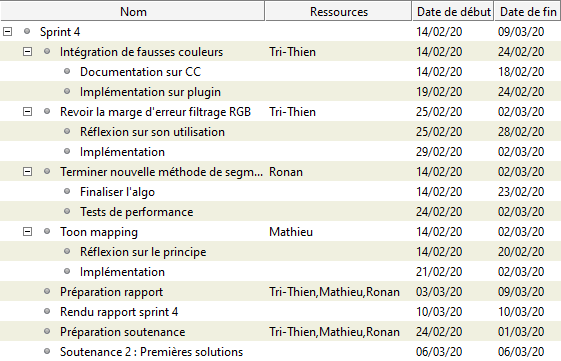
\includegraphics[width=1\textwidth]{./img/sprint_iteration_4_tableau.PNG}
% \raisebox{-1\height}
% {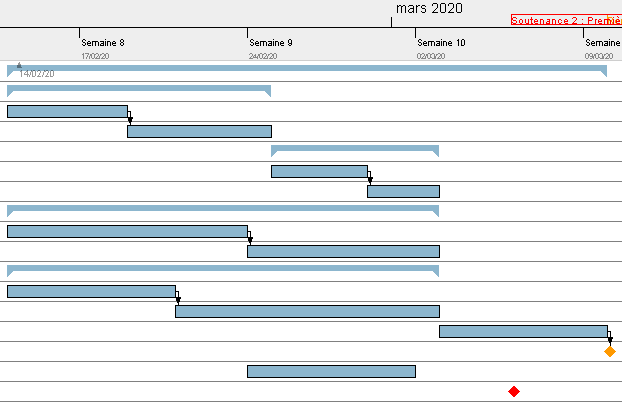
\includegraphics[width=1\textwidth]{./img/sprint_iteration_4_diagramme.PNG}} 
%\end{figure}

\section{Résumé}
\subsection{Tâches principales réalisées dans l'itération}

\subsection{Tâches principales à réaliser pour la prochaine itération}

\begin{thebibliography}{3}


\end{thebibliography}
\end{document}
